\section{Artificial Intelligence\\{\small Paradigmi}} % (fold)
\label{sec:ai_paradigms}
%
\begin{frame}[t,fragile] \frametitle{Intelligenza Artificiale}
{\scriptsize
	\onslide<1->
		\framesubtitle{Secondo il creatore della AI}
		\vspace*{3pt}
		\begin{minipage}[t]{\textwidth}
			\begin{minipage}[t]{0.45\textwidth}
				\centering
				\begin{figure}[ht]
					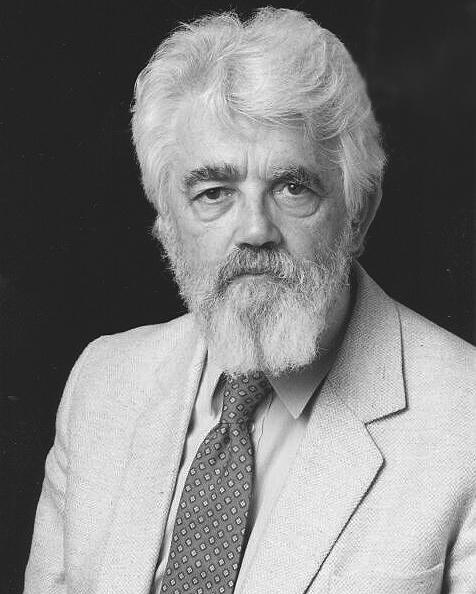
\includegraphics[width=0.73\textwidth]{John-McCarthy.jpg}
					{\tiny\\John McCarthy\\\vspace*{-1pt}\textit{\textcopyright Naukas}}
				\end{figure}
			\end{minipage}
		    \begin{minipage}[t]{0.5\textwidth}
				\renewcommand{\epigraphsize}{\small}
				\setlength{\afterepigraphskip}{0pt}
				\setlength{\beforeepigraphskip}{5pt}
				\setlength{\epigraphwidth}{\textwidth}
				\epigraph{
					\textit{\alert{D:} Cosa è l'Intelligenza Artificiale?\\
					\alert{R:} E' la scienza e l'ingegneria di creare macchine intelligenti, in particolare programmi informatici intelligenti. È correlata al compito simile di utilizzare i computer per comprendere l'intelligenza umana, ma l'intelligenza artificiale non deve limitarsi a metodi che siano osservabili biologicamente.}}{John McCarthy, \textbf{Stanford Uni, 2007}\\Traduzione: \textit{\textcopyright ChatGPT}}
			\end{minipage}
		\end{minipage}
}
	\onslide<2->
	\begin{itemize}[leftmargin=10pt,align=right]
		\item[\alert{\faArrowCircleRight}] Sistema di AI è un termine estremamente inflazionato\ldots 
		\onslide<3->\item[\alert{\faArrowCircleRight}] \ldots anche per sistemi che AI non sono affatto
	\end{itemize}
\end{frame}
%
\begin{frame}[t,fragile] \frametitle{NON Intelligenza Artificiale}
	\vspace*{-15pt}
	\begin{center}
		\begin{minipage}[t]{0.6\textwidth}
			\centering
			\begin{figure}[ht]
				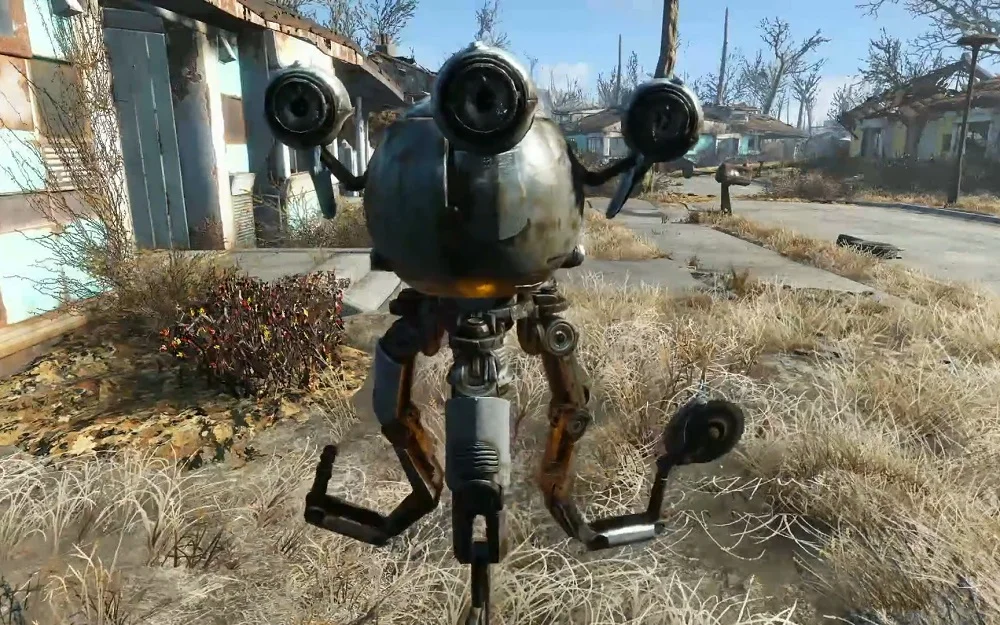
\includegraphics[width=\textwidth]{codsworth.png}
			\end{figure}
		\end{minipage}
		\begin{minipage}[t]{0.6\textwidth}
			\renewcommand{\epigraphsize}{\tiny}
			\setlength{\afterepigraphskip}{0pt}
			\setlength{\beforeepigraphskip}{5pt}
			\setlength{\epigraphwidth}{\textwidth}
			\epigraph{\textit{Questo significa che sei, ehm\ldots in ritardo di due secoli per cena! Forse potrei prepararti uno spuntino? Devi essere affamato!}}{Codsworth all'Unico Sopravissuto, \textbf{Fallout 4, 2015}\\\vspace*{0pt}\textit{\textcopyright Nukapedia: The Fallout Wiki}}
		\end{minipage}
	\end{center}
	\onslide<2->
	\begin{itemize}[leftmargin=10pt,align=right]
		\item[\alert{\faArrowCircleRight}] \alert{\textit{Non-Playable Characters}} (NPC) dei \textit{videogame} 
		\onslide<3->\item[\alert{\faExclamationTriangle}] Sistemi di regole \textit{if-then-else}, \alert{non} AI
	\end{itemize}
\end{frame}
%
\section{AI: Debole vs Forte} % (fold)
\label{sec:ai_types}
%
\begin{frame}[t,fragile] \frametitle{Artificial Intelligence}
	\framesubtitle{Due paradigmi a confronto}
	{\scriptsize
	    \begin{minipage}[t]{\textwidth}
			\begin{minipage}[t]{0.6\textwidth}
	    		\begin{itemize}[leftmargin=10pt,align=right]
					\onslide<1->{\item[\alert{\faArrowCircleRight}] \alert{AI Debole (Narrow AI):} sistemi specializzati per compiti specifici
					\begin{itemize}[leftmargin=10pt,align=right]
						\item[\alert{\faArrowCircleRight}] Contesto \alert{noto a priori}, definito dai dati su cui il sistema è addestrato
						\item[\alert{\faArrowCircleRight}] Incapaci di generalizzare oltre il loro scopo
					\end{itemize}}
					\onslide<2->{\item[\alert{\faArrowCircleRight}] \alert{AI Forte (General AI):} sistemi autonomi e coscienti in grado di affrontare situazioni anche impreviste 
					\begin{itemize}[leftmargin=10pt,align=right]
						\item[\alert{\faArrowCircleRight}] Contesto \alert{dinamico}, definito dalla realtà, interpretato dal sistema
						\item[\alert{\faArrowCircleRight}] Soluzione trovata a fronte di una \alert{comprensione della natura del problema}
						\item[\alert{\faArrowCircleRight}] Creatività e intuizione
					\end{itemize}}					
					\onslide<3->{\item[\alert{\faArrowCircleRight}] \alert{Super AI:} intelligenza che supera quella umana in tutti i domini
					\begin{itemize}[leftmargin=10pt,align=right]
						\item[\alert{\faArrowCircleRight}] Teoria dell'Auton
					\end{itemize}}					
					\onslide<4->{\item[\alert{\faExclamationTriangle}] Oggi esistono \alert{solo} sistemi di AI Debole}
					\begin{itemize}[leftmargin=10pt,align=right]
						\onslide<5->{\item[\alert{\faArrowCircleRight}] Stime GAI: 2040--2060}
					\end{itemize}	
				\end{itemize}
            \end{minipage}
			\begin{minipage}[t]{0.4\textwidth}
				\centering
				\only<1-2|handout:1>{
                	\begin{figure}[ht]
                    	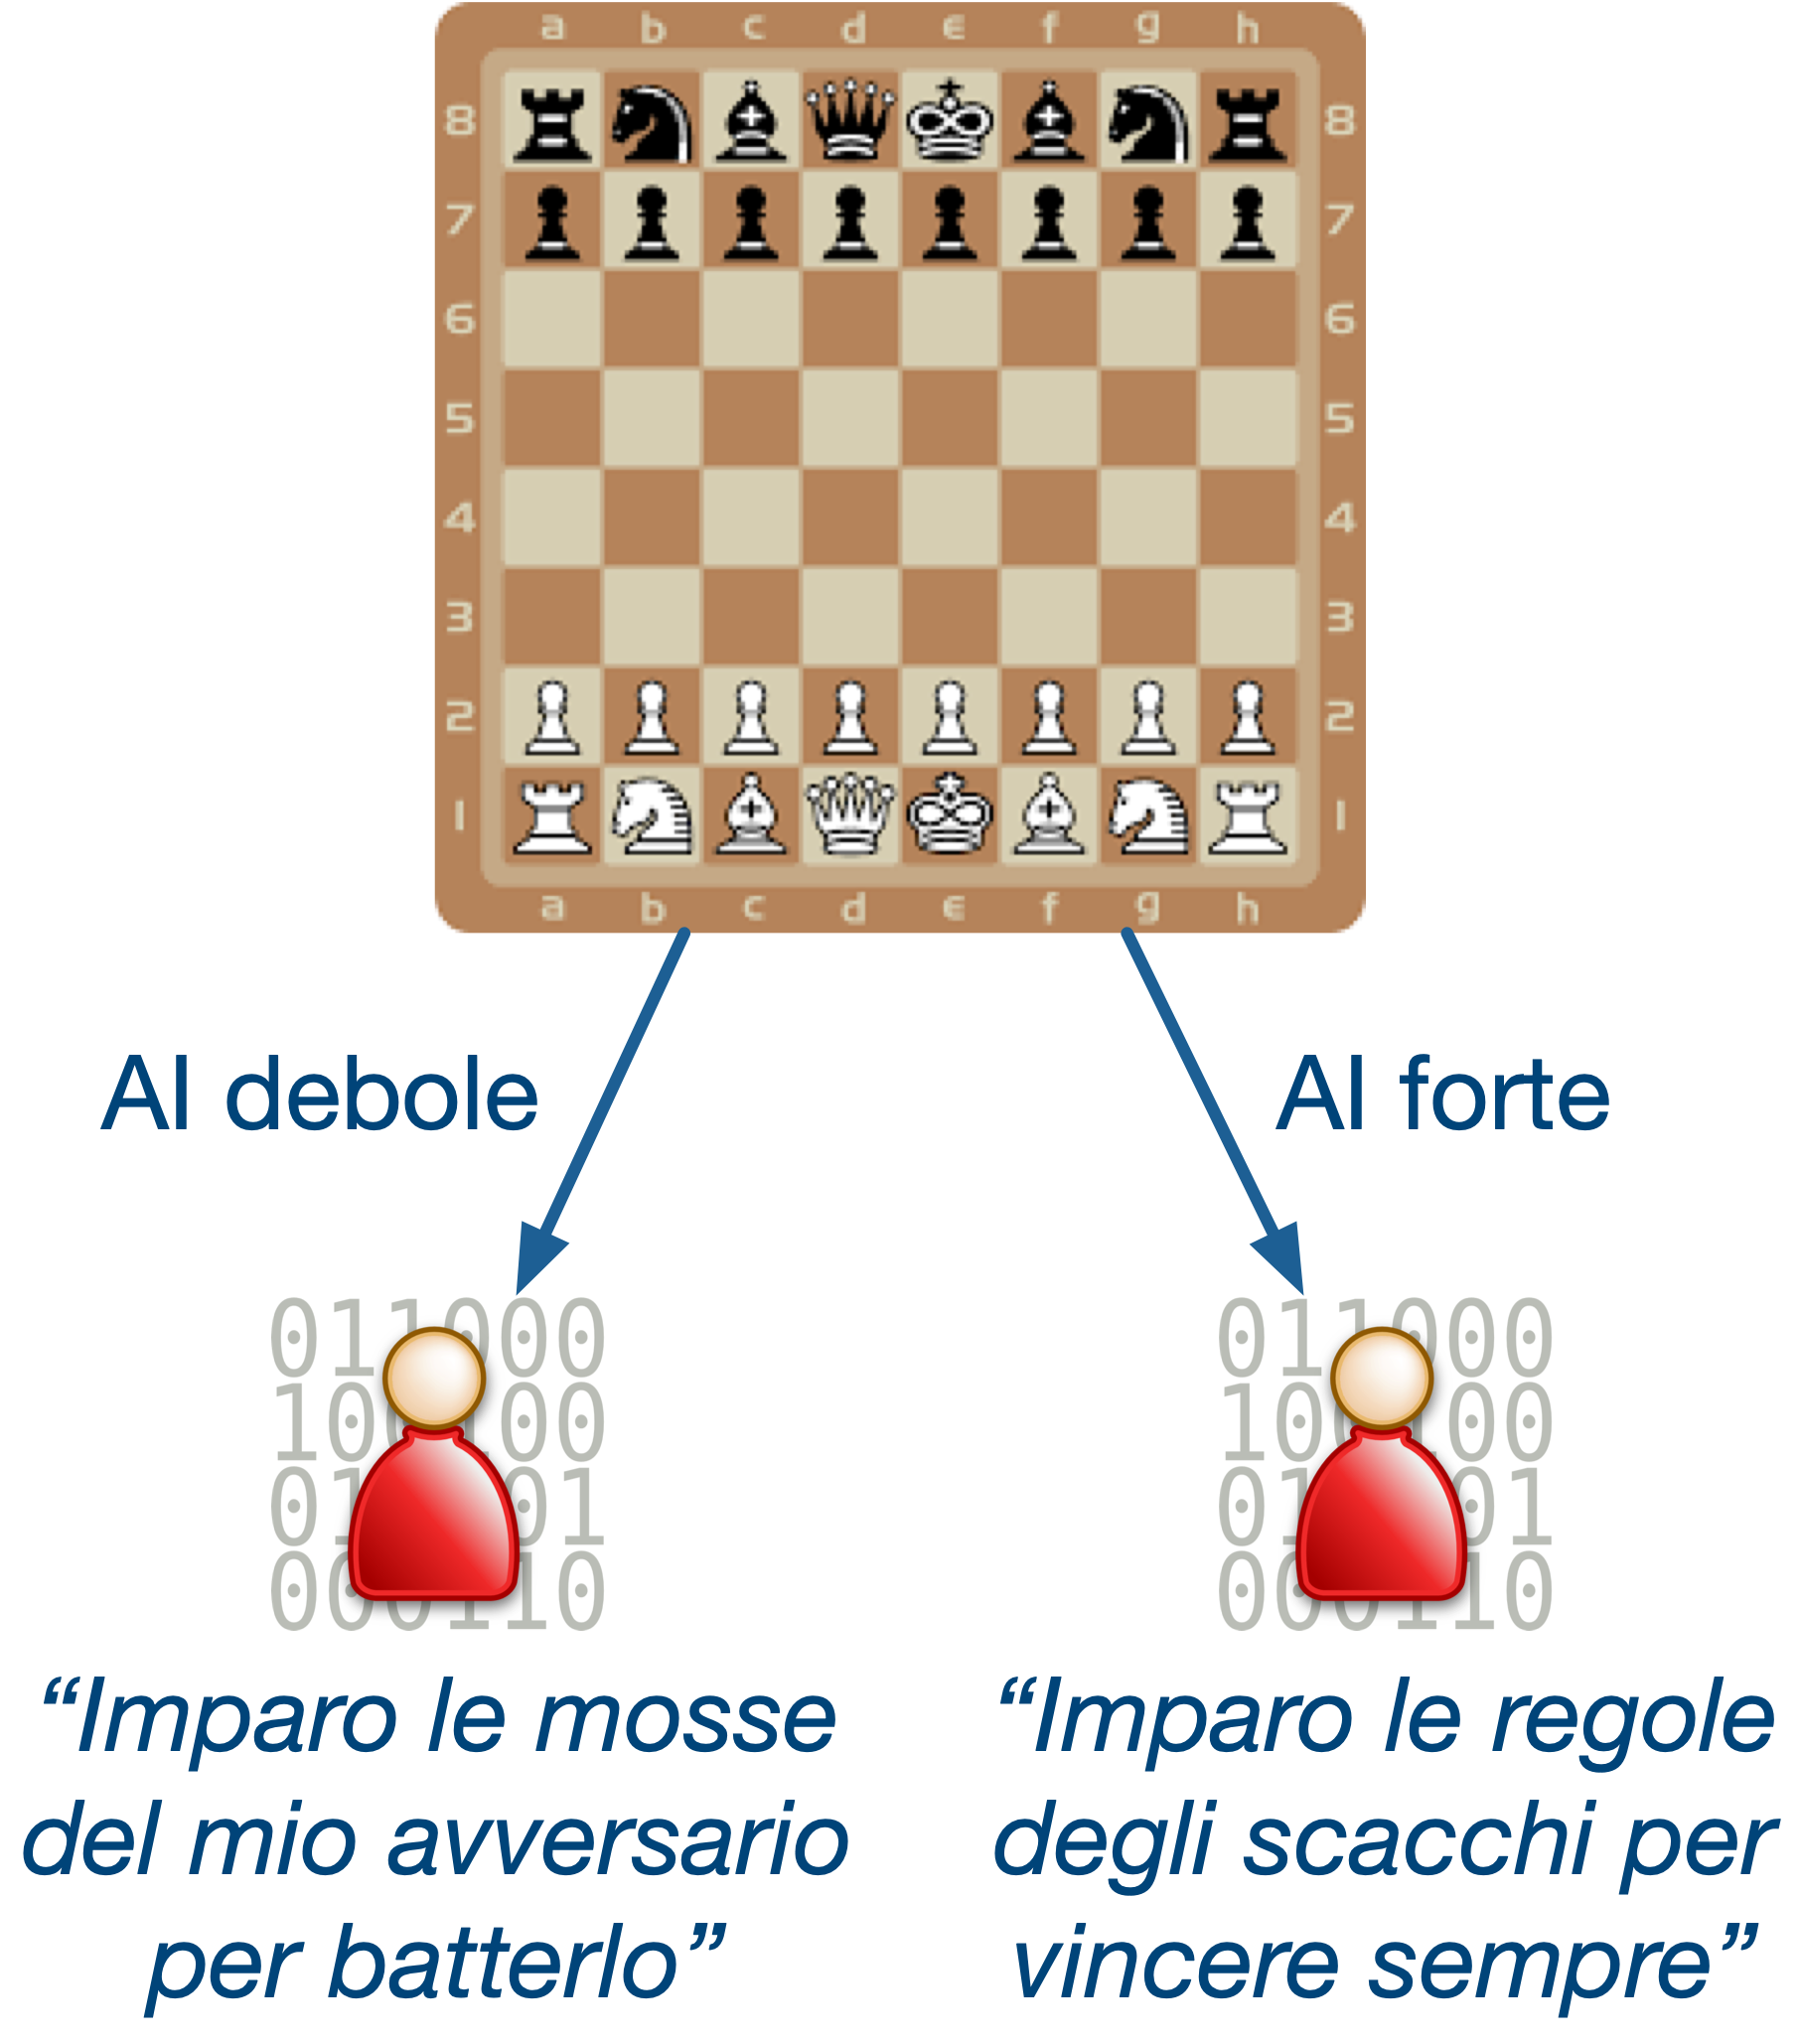
\includegraphics[width=0.8\textwidth]{AI-chess.png}
                    	{\tiny\\Scacchista AI: versione debole e forte\\\textit{\textcopyright Simone Scannapieco}}
                	\end{figure}
				}
				\only<3-5|handout:2>{
                	\begin{figure}[ht]
                    	
\includegraphics[width=0.7\textwidth]{annalee-call.png}
                    	{\tiny\\Annalee Call\\\textbf{AI programmata da sistemi di AI forte}\\\textit{\textcopyright Alien: Resurrection}}
                	\end{figure}
				}
	    	\end{minipage}
		\end{minipage}
	}
\end{frame}
%
\begin{frame}[t,fragile] \frametitle{AI debole: esempi}
	\framesubtitle{Casi d'uso}
		\begin{itemize}[leftmargin=10pt,align=right]
			\item[\alert{\faArrowCircleRight}] \alert{Analisi del \textit{sentiment}:} classificare recensioni dei clienti
		\end{itemize}
		\vspace*{.3cm}
		\begin{shellcodeblock}{Analizzatore \textit{sentiment} (\textcopyright\ Claude)}
        	\begin{minted}{java}
    @RestController
    public class SentimentController {

        @Autowired
        private SentimentAnalysisService service;

        @PostMapping("/analyze")
        public SentimentResult analyze(@RequestBody String text) {
            return service.analyzeSentiment(text);
        }
    }
			\end{minted}
    	\end{shellcodeblock}
\end{frame}
%
\begin{frame}[t,fragile] \frametitle{AI debole: esempi}
	\framesubtitle{Casi d'uso}
		\begin{itemize}[leftmargin=10pt,align=right]
			\item[\alert{\faArrowCircleRight}] \alert{\textit{Chatbot} per supporto:} rispondere a domande frequenti
		\end{itemize}
		\vspace*{.3cm}
    	\begin{shellcodeblock}{\textit{Chatbot} tradizionale con regole fisse (\textcopyright\ Claude)}
        	\begin{minted}{java}
    @Component
    public class ChatbotService {

        public String processQuery(String userQuery) {
            if (userQuery.contains("password")) {
                return "Per resettare la password...";
            }
            // Pattern matching limitato
            return "Non ho capito la domanda";
        }
    }
			\end{minted}
    	\end{shellcodeblock}
\end{frame}
%
\begin{frame}[t,fragile] \frametitle{AI debole: esempi}
	\framesubtitle{Casi d'uso}
		\begin{itemize}[leftmargin=10pt,align=right]
			\item[\alert{\faArrowCircleRight}] \alert{Rilevamento frodi:} identificare transazioni sospette
		\end{itemize}
		\vspace*{.3cm}
    	\begin{shellcodeblock}{Sistema di rilevamento frodi basato su ML (\textcopyright\ Claude)}
        	\begin{minted}{java}
    @Service
    public class FraudDetectionService {
    
        public boolean isFraudulent(Transaction tx) {
            // Analizza pattern: importo, orario, 
            // geolocalizzazione, frequenza
            return mlModel.predict(tx.getFeatures()) > 0.8;
        }
    }
			\end{minted}
    	\end{shellcodeblock}
\end{frame}
%
\begin{frame}[t,fragile] \frametitle{AI debole: esempi}
	\framesubtitle{Casi d'uso}
		\begin{itemize}[leftmargin=10pt,align=right]
			\item[\alert{\faArrowCircleRight}] \alert{Rilevamento frodi:} identificare transazioni sospette
		\end{itemize}
		\vspace*{.3cm}
    	\begin{shellcodeblock}{\textit{Pricing} dinamico basato su AI (\textcopyright\ Claude)}
            \begin{minted}{java}
    @RestController
    public class PricingController {
    
        @Autowired
        private DynamicPricingService pricingService;

        @GetMapping("/price/{productId}")
        public PriceResponse getPrice(@PathVariable Long productId,
                                      @RequestParam String customerSegment) {
            return pricingService.calculateOptimalPrice(productId,
                                                        customerSegment);
        }
    }
			\end{minted}
    	\end{shellcodeblock}
\end{frame}
%
\begin{frame}[t,fragile] \frametitle{AI Forte: Esempi Ipotetici}
	\framesubtitle{Cosa potrebbe fare un'AGI}
	{\small
		\begin{itemize}[leftmargin=10pt,align=right]
			\onslide<1->{\item[\alert{\faArrowCircleRight}] \alert{Programmatore universale:} scrivere codice in qualsiasi linguaggio e dominio}
			\onslide<2->{\item[\alert{\faArrowCircleRight}] \alert{\textit{Problem solver} generale:} risolvere problemi mai visti prima}
			\onslide<3->{\item[\alert{\faArrowCircleRight}] \alert{Apprendimento rapido:} imparare nuovi concetti da pochi esempi}
			\onslide<4->{\item[\alert{\faArrowCircleRight}] \alert{Ragionamento causale:} comprendere cause ed effetti complessi}
		\end{itemize}
		\vspace*{.3cm}
		\hspace*{4cm}
		\only<1|handout:1>{
		\begin{minipage}[t]{\textwidth}
			\begin{minipage}[t]{0.6\textwidth}
				\renewcommand{\epigraphsize}{\scriptsize}
				\setlength{\afterepigraphskip}{0pt}
				\setlength{\beforeepigraphskip}{5pt}
				\setlength{\epigraphwidth}{0.9\textwidth}
				\epigraph{\textit{Analizzerò il tuo sistema legacy in COBOL, lo convertirò in microservizi Spring Boot, ottimizzerò le performance del database, implementerò la sicurezza OAuth2 e creerò una UI React responsive. Tutto completato in 30 minuti.}}{Scenario ipotetico di AGI programmatore}
			\end{minipage}
		\end{minipage}
		}
		\only<2|handout:2>{
		\begin{minipage}[t]{\textwidth}
			\begin{minipage}[t]{0.6\textwidth}
				\renewcommand{\epigraphsize}{\scriptsize}
				\setlength{\afterepigraphskip}{0pt}
				\setlength{\beforeepigraphskip}{5pt}
				\setlength{\epigraphwidth}{0.9\textwidth}
				\epigraph{\textit{Il tuo e-commerce ha un calo delle vendite del 23\%. Dopo aver analizzato dati di mercato, comportamento utenti e tendenze sociali, ho identificato 12 fattori causali e propongo una strategia integrata che combina UX, pricing e marketing personalizzato.}}{Scenario di problem solving generale}
			\end{minipage}
		\end{minipage}
		}
		\only<3|handout:3>{
		\begin{minipage}[t]{\textwidth}
			\begin{minipage}[t]{0.6\textwidth}
				\renewcommand{\epigraphsize}{\scriptsize}
				\setlength{\afterepigraphskip}{0pt}
				\setlength{\beforeepigraphskip}{5pt}
				\setlength{\epigraphwidth}{0.9\textwidth}
				\epigraph{\textit{Non ho mai visto il framework Quantum-Spring che avete appena rilasciato, ma dopo aver letto 3 esempi di codice ho compreso i pattern architetturali e posso già ottimizzare la vostra implementazione.}}{Apprendimento rapido da pochi esempi}
			\end{minipage}
		\end{minipage}
		}
		\only<4|handout:4>{
		\begin{minipage}[t]{\textwidth}
			\begin{minipage}[t]{0.6\textwidth}
				\renewcommand{\epigraphsize}{\scriptsize}
				\setlength{\afterepigraphskip}{0pt}
				\setlength{\beforeepigraphskip}{5pt}
				\setlength{\epigraphwidth}{0.9\textwidth}
				\epigraph{\textit{Il bug nel vostro sistema non è dove pensate. Il vero problema è un race condition causato da un pattern di design che crea dipendenze cicliche tra tre microservizi, amplificato dal garbage collector di JVM sotto carico elevato.}}{Ragionamento causale profondo}
			\end{minipage}
		\end{minipage}
		}
	}
\end{frame}
%
\begin{frame}[t,fragile] \frametitle{Confronto: AI Debole vs AI Forte}
	{\small
		\framesubtitle{Differenze pratiche per lo sviluppatore}
		\vspace*{-.5cm}
		\begin{center}
		{\scriptsize
		\begin{table}
			\setlength{\tabcolsep}{4pt}
			\renewcommand{\arraystretch}{1.5}
			\centering
			\begin{tabularx}{\textwidth}{p{2cm}XX}
				\toprule
				\textbf{Aspetto} & \textbf{AI Debole (Narrow)} & \textbf{AI Forte (General)}\\
				\midrule
				\alert{Scopo} & Un singolo compito specifico & Qualsiasi compito cognitivo\\
				\alert{Apprendimento} & Dataset grandi, training lungo & Pochi esempi, apprendimento rapido\\
				\alert{Trasferibilità} & Zero (limitata al dominio) & Totale (tra qualsiasi dominio)\\
				\alert{Creatività} & Assente o molto limitata & Creatività genuina\\
				\alert{Ragionamento} & Pattern matching avanzato & Comprensione causale\\
				\alert{Implementazione} & Disponibile oggi & Non esiste ancora\\
				\alert{Costo/Complessità} & Gestibile per singoli casi d'uso & Teoricamente enorme\\
				\bottomrule
			\end{tabularx}
		\end{table}
		}
		\end{center}
	}
\end{frame}
%